\artikkelopener{Fantastisk sesong – og et varselskudd}{Norsk friidrett står sterkt akkurat nå. Men hva skjer når dagens medaljører legger opp?}{Henning Hofstad}{Fagnytt 1 · 2026}{Redaktørens corner}{Vi kan glede oss over en sesong med fantastiske prestasjoner. Samtidig er det god grunn til å være bekymret for nivået i de tekniske øvelsene og i yngste juniorklasse.}

\begin{wrapfigure}{r}{27mm}
\vspace{-10pt}
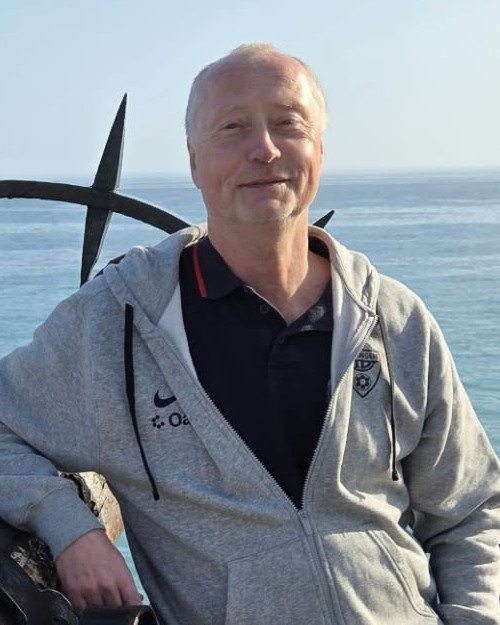
\includegraphics[width=27mm]{blad/bilder/henning_hofstad.jpg}\\[2pt]
{\raggedright\kickfont\scriptsize\color{lysgra}HENNING HOFSTAD\\REDAKTØR\par}
\vspace{-10pt}
\end{wrapfigure}

Når en ser på den nå avsluttede sesongen, kan en se på den med forskjellige blikk. Vi kan glede oss over de fantastiske prestasjonene til Henriette Jæger, Jakob Ingebrigtsen, Karsten Warholm, Sondre Guttormsen, Beatrice Llano og Anthony Ommundsen Johnsen og glede oss over at Sander Skotheim og Markus Rooth er tilbake etter skader. Sander sågar med medalje til tross for at han lå en del under toppnivå. Vi kan samtidig være bekymret over tilstanden i mange av de tekniske øvelsene. Det er også god grunn til å være bekymret over nivået generelt i yngste juniorklasse.

Norges forrige storhetsperiode som friidrettsnasjon endte med en gedigen nedtur da alle de fremste utøverne gav seg etter OL i 2000. En tiårsperiode bar Andreas Thorkildsen norsk friidrett neste alene. Hvorfor skjedde dette? Her kan en peke på at masse ressurser ble brukt på topputøverne og at juniorsektoren ble for lavt prioritert inn mot årtusenskiftet. Det var rett og slett få eller ingen til å ta over. Det kan også skyldes tilfeldigheter, at akkurat da hadde ikke Norge utøveren med de genetiske kvalitetene som er nødvendig for å nå internasjonal topp.

I øyeblikket står norsk friidrett svært sterkt, men kan det samme skje igjen? At når dagens generasjon av medaljører avslutter karrieren sin, så er det få eller ingen nye medaljører på gang?

Det er meget tenkbart. Etter å ha studert junior-NM og UM må en innse at det ikke er noen, bortsett fra Anthony, som dominerer slik Karsten, Jakob, Sander, Karoline Grøvdal og Henriette gjorde i junioralder. Kan det skje at Anthony på et tidspunkt blir en ensom svale i verdenstoppen?

\begin{sitat}

«Det kreves tiltak for å heve nivået på juniorsiden, særlig i tekniske øvelser.»

\end{sitat}

En kan med rette stille spørsmål om det er nødvendig å holde så høyt nivå som junior for å komme verdenseliten. Unntak finnes alltid. Sondre Guttormsen er et eksempel på dette. Han var god, men ikke ekstremt god, som junior og har maktet å heve seg til å bli en av verdens 3-4 beste stavhoppere i dag. Uansett viser statistikken at det er en nødvendighet å være til stede under juniormesterskapene. En trenger ikke ta medalje, men en bør ha det internasjonale nivået inne som junior dersom en skal ta medaljer i seniorklassen. I år hadde vi ingen finalister i tekniske øvelser i de internasjonale juniormesterskapene, noen få i løp plasserte seg blant de 12 beste.

Det kreves tiltak for å heve nivået på juniorsiden, særlig i tekniske øvelser. Dette er tatt opp i artikkelen; «Hvor forsvant alle høydehopperne?».

Norge er et lite land med få innbyggere. Klimaet er heller ikke det beste for friidrett. Hvordan kan det så ha seg at utøvere fra Norge har vunnet gull i verdensidretten friidrett under seks av de åtte siste olympiske leker, med seks forskjellige utøvere? Ser en på Norge som et lag er det en utrolig lagprestasjon.

Det er akseptert at det kreves helt spesielle genetiske egenskaper for å nå til topps i internasjonal friidrett. Hvis en ser på genetiske egenskaper kun som iboende fysiske egenskaper skulle det være statistisk umulig for Norge med sitt innbyggertall å ha så mange utøvere i verdenseliten. En bør derfor se på genetiske egenskaper i videre forstand. En kan se på gener som et viktig grunnlag, men som det er mulig å forvalte på best mulig måte.

Kvaliteten på denne forvaltningen gir svaret på hvorfor Norge stadig har utøvere i verdenstoppen. Igjen et bevis på den høye standarden det er på norske trenere.

Til sist vil jeg gi en honnør til Reidar Langkjær. Han har stilt sine bilder til disposisjon for Fagnytt uten vederlag og er alltid positiv til å bidra til det beste for bladet.

\sluttmerke
